\documentclass[letterpaper, 11 pt, conference]{ieeeconf} 

\usepackage[english]{babel}
\usepackage[utf8]{inputenc}
\usepackage{amsmath}
\usepackage{graphicx}
\usepackage[colorinlistoftodos]{todonotes}
\usepackage[margin=1in, top=0.5in]{geometry}
\usepackage{hyperref}

\title{ORIE 4741: Final Project Report \\
\large Restaurant Inspection Prediction with Yelp Reviews in Las Vegas}

\author{\textit{Yuyang Chen (yc2324), Xinyun Tang (xt222), Xiaoxi Zhang (xz577)}}
\date{\today}

\begin{document}
\maketitle

%%%%%%%%%%%%%%%%%%%%%%%%%%%%%%%%%%%%%%%%%%%%%%%%%%%%%%%%%%%%%%%%%%%%%%%%%%%%%%%%
\begin{abstract}
Restaurant inspection plays an important role in
customers' daily life and restaurant business. Yelp.com, on the other hand, is a popular social media platform that influences customers' choices of restaurants everyday. To raise public awareness
on food safety problems, we used restaurant features from Yelp.com and City Department of Health to build the prediction model of restaurants' health inspection results based on 1924 restaurants in Las Vegas. We compared linear models with Huber, Quadratic loss function and quadratic and L1 regularizers, along with non-linear models (i.e. random forest and gradient boosted model). The results indicated that gradient boosted model with quantile loss function is the most suitable model in the context of predicting restaurants' health inspection results and providing a guidance for healthy dining. 

\end{abstract}
%%%%%%%%%%%%%%%%%%%%%%%%%%%%%%%%%%%%%%%%%%%%%%%%%%%%%%%%%%%%%%%%%%%%%%%%%%%%%%%%


%%%%%%%%%%%%%%%%%%%%%%%%%%%%%%%%%%%%%%%%%%%%%%%%%%%%%%%%%%%%%%%%%%%%%%%%%%%%%%%%
\section*{1 Data Acquisition}

\subsection*{1.1 Inspection Datasets}

The health inspection dataset comes from LasVegasNeveda.gov and contains basic information about the restaurant and details about the inspection result history. Each inspection record includes the number of demerits, type of inspection, inspection grade, violations, inspection time, etc. We used the average number of past violations as the dependent variable. 

%%%%%%%%%%%%%%%%%%%%%%%%%%%%%%%%%%%%%%%%%%%%%%%%%%%%%%%%%%%%%%%%%%%%%%%%%%%%%%%%

\subsection*{1.2 Yelp Dataset}

By web scrapping, we fetched data directly from restaurants' Yelp pages. Yelp reviews are very informative. For each restaurant, we obtained the first 400 reviews (20 pages) on their Yelp web page. In addition to capturing review content, we also recorded dates of the review, "usefulness" of the review evaluated by other users, and review star ratings, review counts (i.e. how many reviews a restaurant has in total). General restaurant information such as expensive rating, overall star rating and neighborhood were also obtained through web scraping. In the end, we were able to obtain 623,602 reviews from 1924 restaurants. which is approximately 324 reviews per restaurant. 

%%%%%%%%%%%%%%%%%%%%%%%%%%%%%%%%%%%%%%%%%%%%%%%%%%%%%%%%%%%%%%%%%%%%%%%%%%%%%%%%

%%%%%%%%%%%%%%%%%%%%%%%%%%%%%%%%%%%%%%%%%%%%%%%%%%%%%%%%%%%%%%%%%%%%%%%%%%%%%%%%
\section*{2 Data Cleaning and Feature Engineering}

\subsection*{2.1 Inspection Dataset Cleanup}

The inspection dataset contains more than 48,000 inspection records conducted by Department of Health for 1924 restaurants. Each restaurants have different numbers of inspection records. To retrieve the variable that represents the overall performance on health level, we have multiple choices: demerits, grades and number of violations. Demerits and grades are both derived from specific violations of restaurants. We chose the averaged number of violations as the dependent variable in our model. Then we computed the following features using inspection records for each restaurant.

\begin{itemize}
\item Re-inspection ratio. Re-inspection processes are usually conducted to recheck the restaurants that performs bad in last inspection. So we calculated the ratio of re-inspection type over the inspection records as a feature in the model. Scatter plot in Figure 1 displays the positive relationship between the re-inspection ratio and averaged violation counts.
\item Grade A ratio. Inspection grades of restaurants represent the accumulative performance of restaurants. Grades might not have a direct relationship with number of violations because Grade-A restaurants may have some violations within certain tolerance. But long-term grade tells a story for the accumulative performance of restaurants. From Figure 1, Grade A ratio has negative relationship with averaged violation counts. 
\end{itemize}

The above two features both have larger variations at restaurants with less than 4 violations. This further implies that the inspection grade is accumulative performance of restaurant so that past grades of restaurants are not robust enough to build the prediction model. This also motivated us to add Yelp datasets in the model. 

\begin{figure}[h]
	\centering
    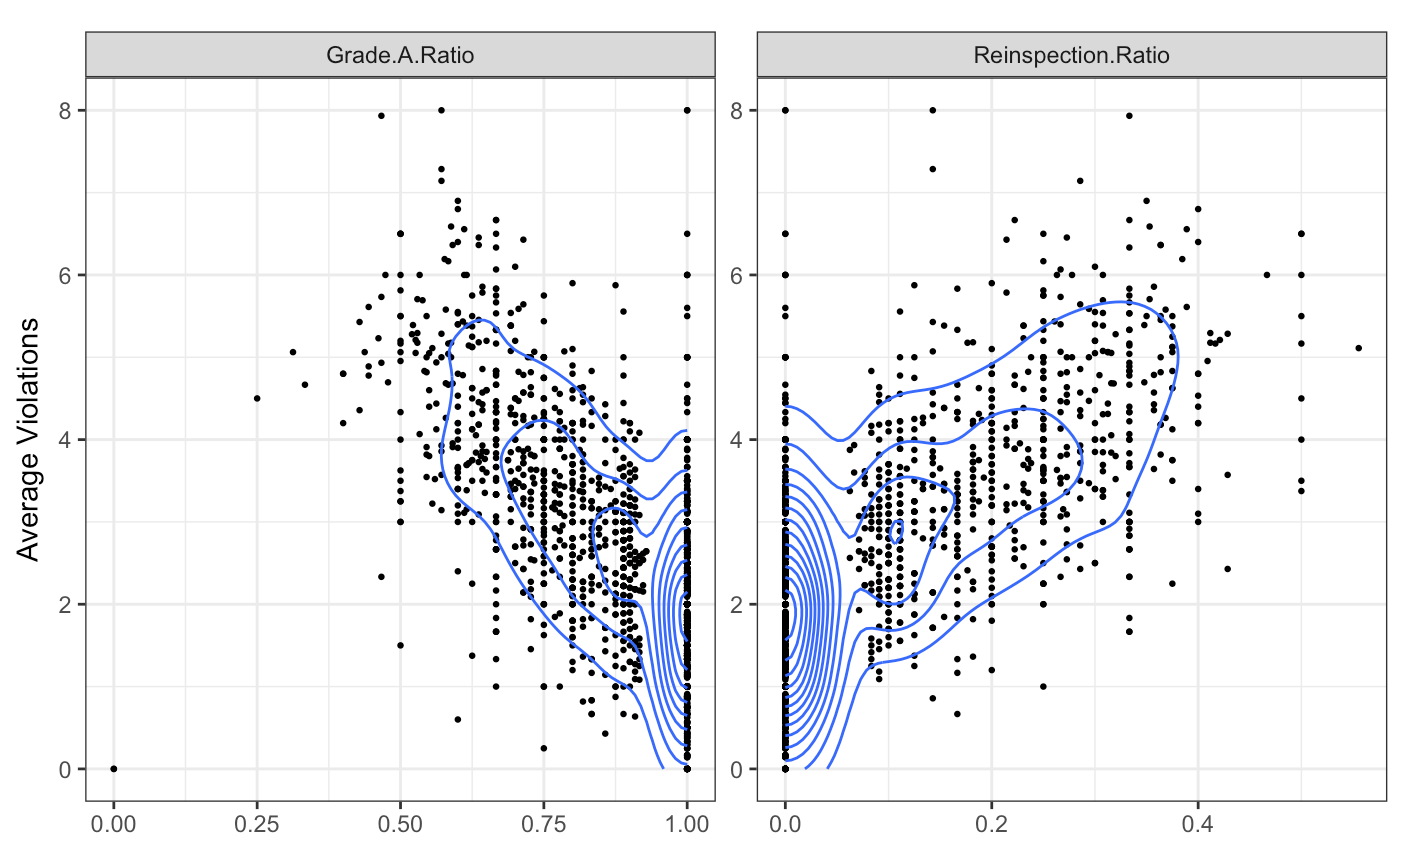
\includegraphics[scale = 0.28]{grade_reinsp}
    \caption{The scatter plot of averaged violation counts and grade A ratio and re-inspection ratio.}
\end{figure}

%%%%%%%%%%%%%%%%%%%%%%%%%%%%%%%%%%%%%%%%%%%%%%%%%%%%%%%%%%%%%%%%%%%%%%%%%%%%%%%%
\subsection*{2.2 Restaurant Features}

\subsection*{2.2.1 Locations}

Locations information of restaurants may relate to the averaged income of people in that area, the level of the restaurants, the cleanness of certain neighborhoods, etc. There are three location variables in the dataset, Longitude, latitude and neighborhood. It's not reasonable to use longitude and latitude in the linear models because we didn't observe trends along latitude and longitude. But we considered them in the non-linear model because non-linear interactions of those two features are important according to some clusters of restaurants with high violation counts in Figure 2. 

The neighborhood information was scrapped from Yelp.com. Certain neighborhoods (e.g. Southeast and East side) has a strong tendency towards larger numbers of violations. There are about 20\% of missing values in neighborhood. By using the zip code of restaurants with missing neighborhood and matching them with nearby restaurants, we filled the about 80\% of the missing data. One-hot-encoding was used to create 15 features for neighborhood.

\begin{figure}[h]
	\centering
    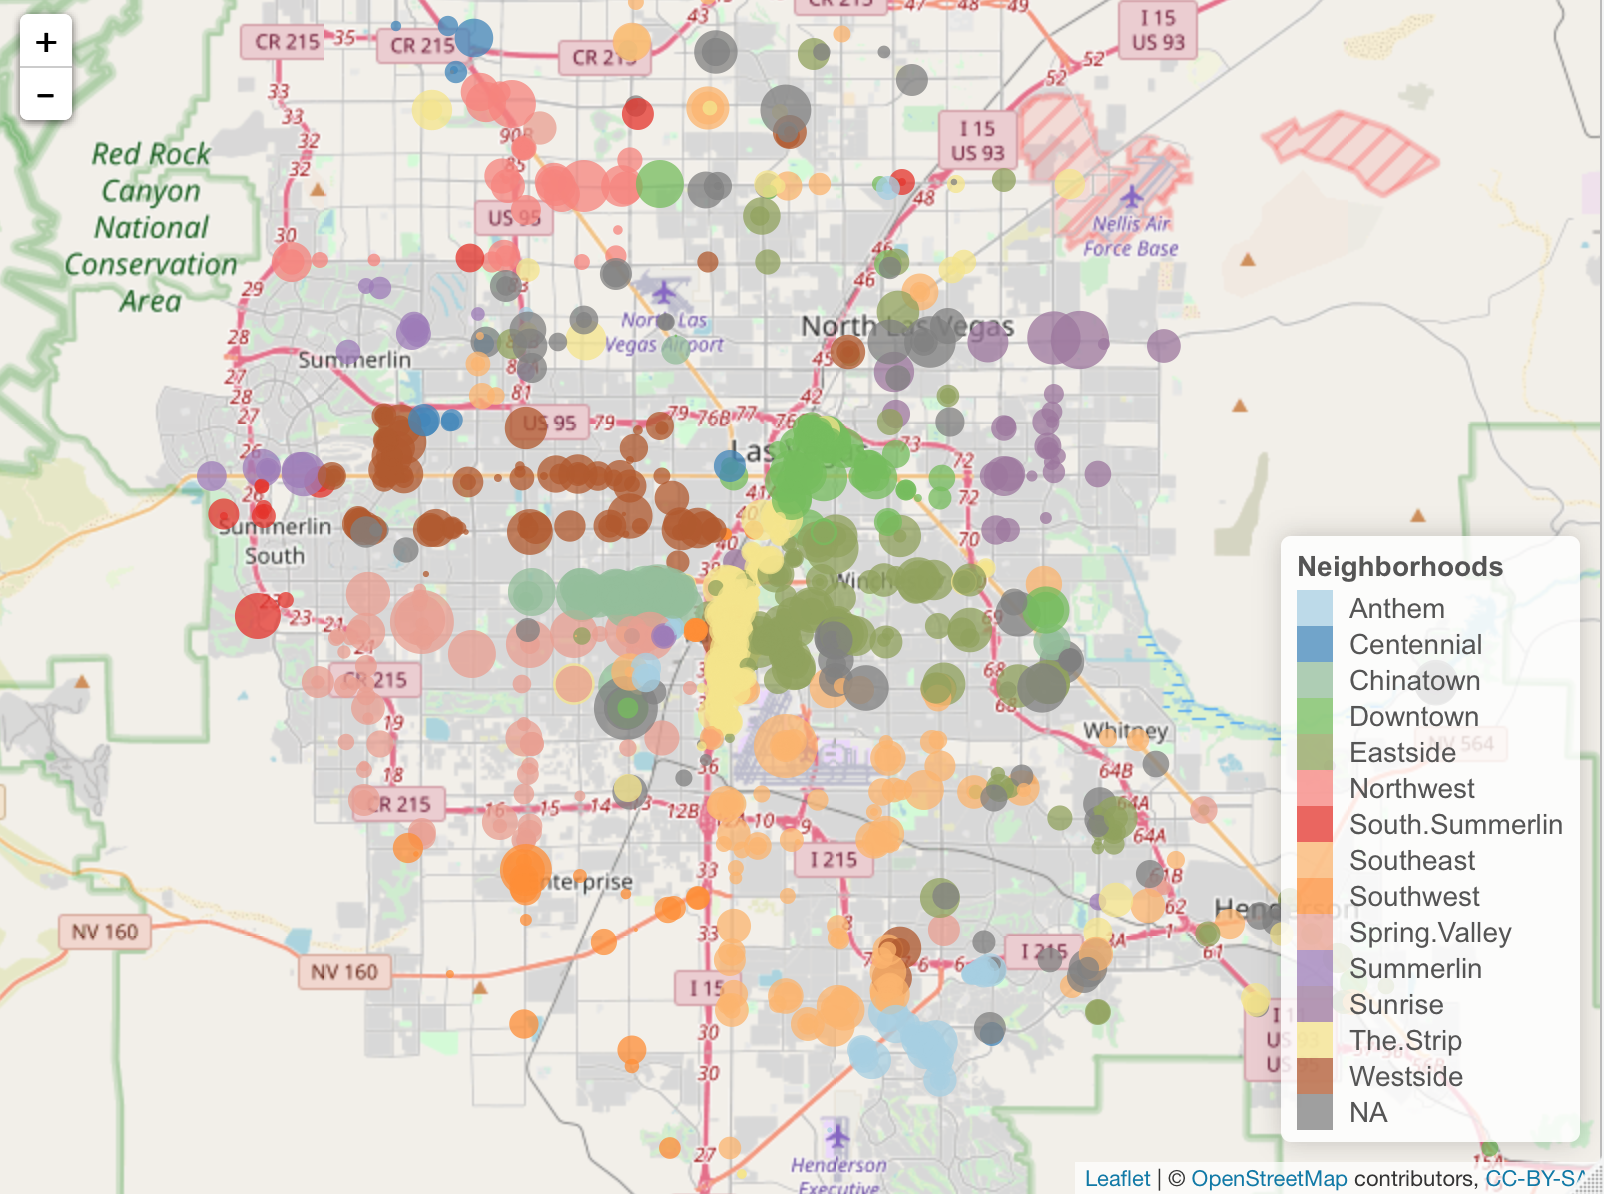
\includegraphics[scale = 0.28]{map_vio}
    \caption{The map of restaurants analyzed in the model in Las Vegas. The restaurants are colored by neighborhood and sized by the averaged violation counts.}
\end{figure}

%%%%%%%%%%%%%%%%%%%%%%%%%%%%%%%%%%%%%%%%%%%%%%%%%%%%%%%%%%%%%%%%%%%%%%%%%%%%%%%%
\subsection*{2.2.2 Restaurant Category}

The restaurant categories from Yelp.com are diverse and detailed. We reclassify over 200 categories into 9 category groups: Asian, Bar, Dessert, Fast food, French, Indian, Italian, Mexican and others. The reclassification strategy is to group similar types of categories. For example, we grouped Chocolate Tiers, Ice Cream Bars and Bakings into dessert. According to the boxplot in Figure 3, Asian and Mexican restaurants have higher median violation counts than other categories. 'Others' category has very high variation due to more restaurants than others. One-hot-encoding was used to create 9 features for categories.

\begin{figure}[h]
	\centering
    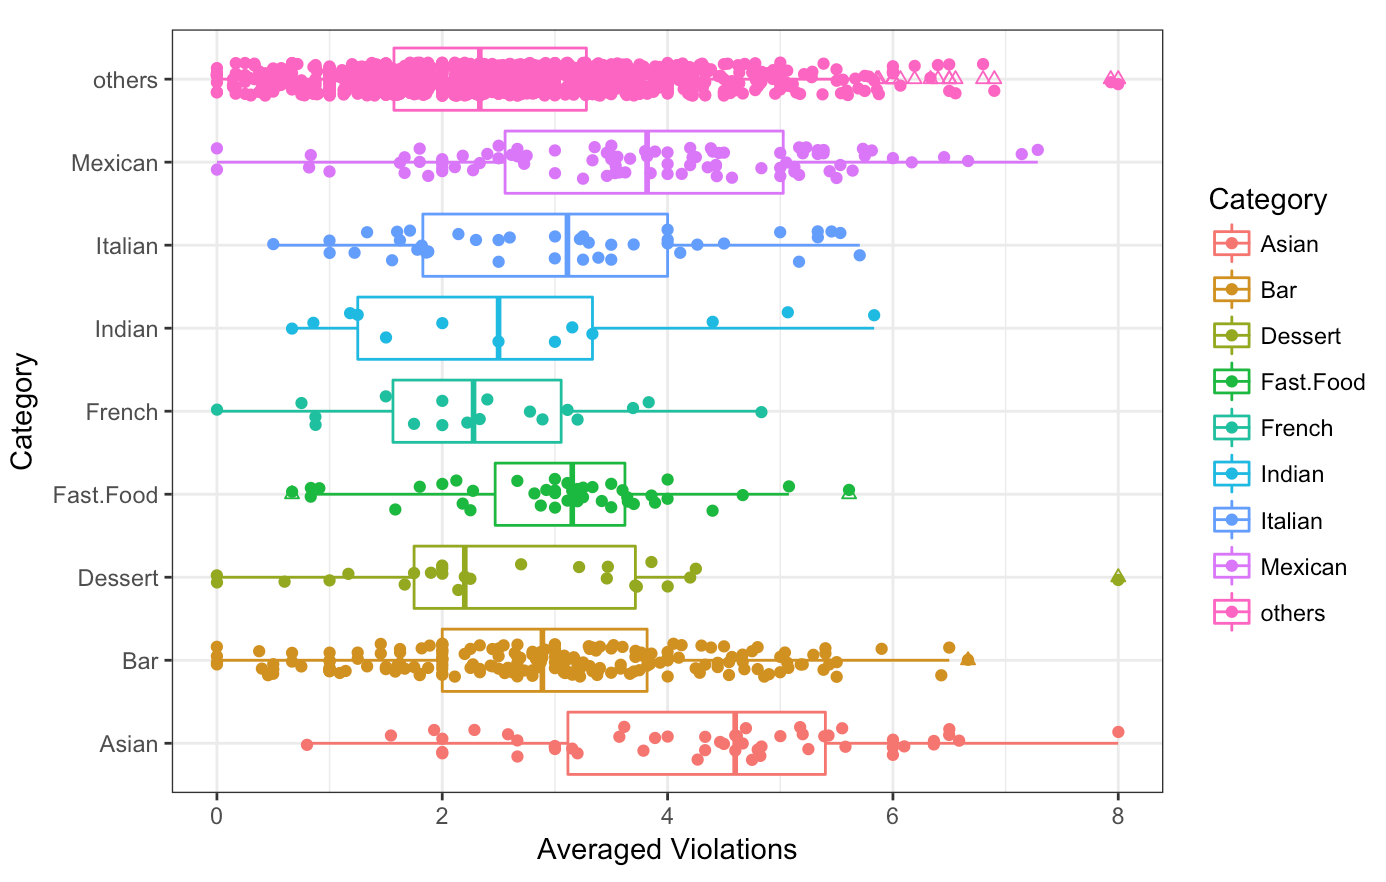
\includegraphics[scale = 0.3]{category}
    \caption{The boxplot of averaged violation counts by categories.}
\end{figure}

%%%%%%%%%%%%%%%%%%%%%%%%%%%%%%%%%%%%%%%%%%%%%%%%%%%%%%%%%%%%%%%%%%%%%%%%%%%%%%%%
\subsection*{2.2.3 Yelp Rating}

The most famous feature that Yelp.com provides is Yelp rating for restaurants. People tend to check the ratings of the restaurants before they decide on which restaurant to go. But is Yelp rating a good representation of restaurants' health level? From the information scrapped from Yelp.com, we retrieved the 'Overall ratings' for each restaurant and crafted a more reasonable rating feature 'Review ratings'. The 'Review ratings' were the weighted mean of reviewers' ratings using the length of their reviews and the usefulness (using the 'Useful' feature from Yelp) of the reviews as weights. That is, we are more confident on reviewers' ratings if the length of the reviews are longer and if they are endorsed by other Yelp users. We compare the two rating features with Averaged Violations in Figure 4. We observed better relationship between averaged violation counts and log transformation of 'Review ratings' than that with Yelp's 'Overall ratings'. Therefore, we used 'Review ratings' instead of Yelp's 'Overall ratings' in our models.

\begin{figure}[h]
	\centering
    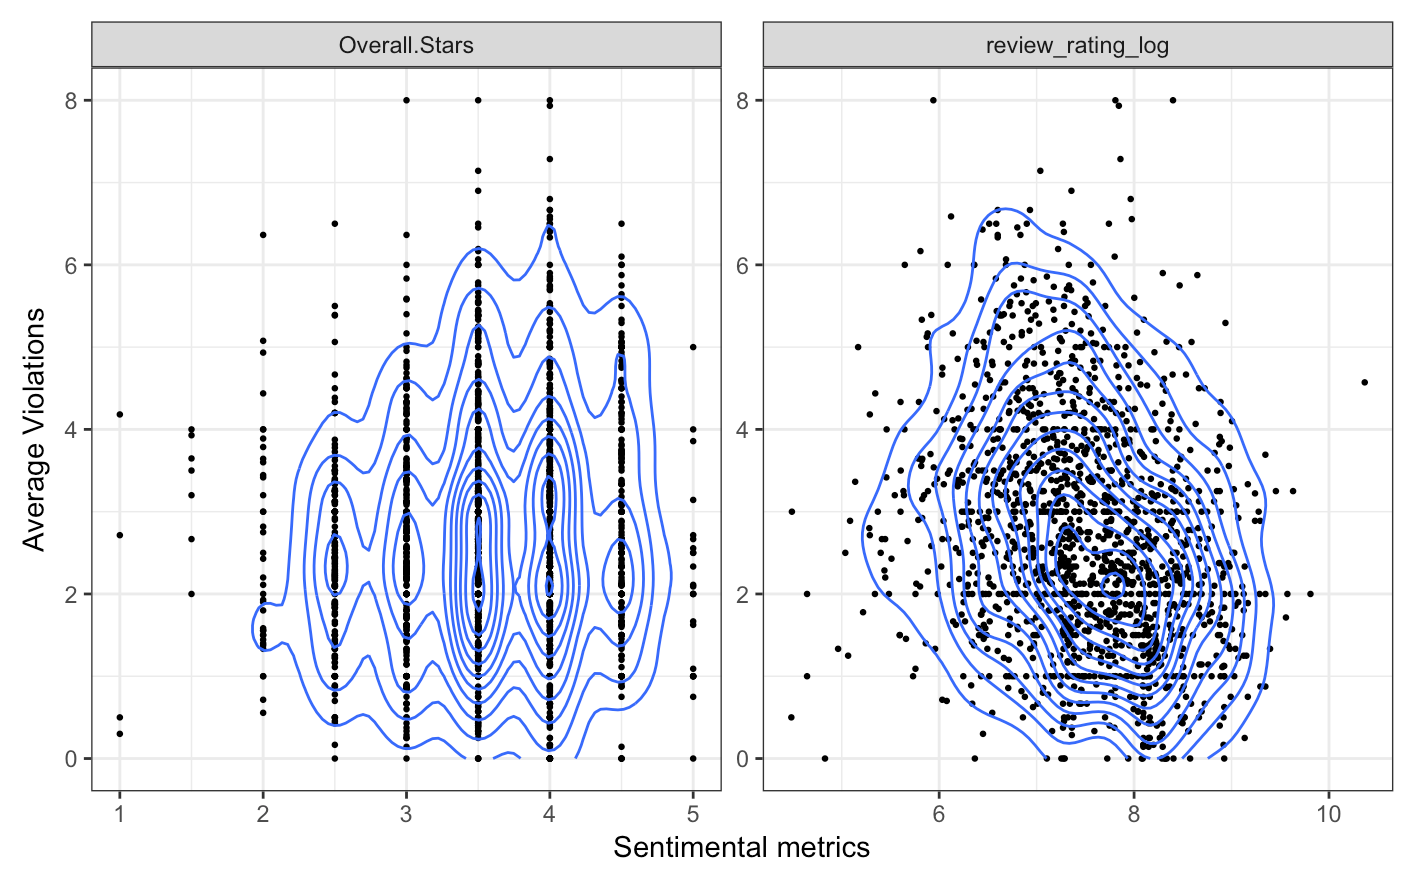
\includegraphics[scale = 0.3]{ratings}
    \caption{The relationship between 'Overall Rating' and log transformation of 'Review Rating' and averaged violation counts. }
\end{figure}

%%%%%%%%%%%%%%%%%%%%%%%%%%%%%%%%%%%%%%%%%%%%%%%%%%%%%%%%%%%%%%%%%%%%%%%%%%%%%%%%
\subsection*{2.2.4 Expensiveness and Popularity}

Yelp.com provides 'dollar sign' for each restaurant, which is the Yelp user's rating on the expensiveness of restaurants. Unlike the overall rating, this feature is trusted by most people. The missing data were replaced by the median value here. According to Figure 5, most restaurants with one dollar sign (cheapest) have more than 2 violations. Restaurants with two dollar signs have approximately symmetric distribution in violation counts. Restaurants with more than 2 dollar signs rarely have more than 4 violations. So the 'dollar sign' feature will be used in the models.

The popularity of restaurants is well represented by the number of reviews on Yelp. We found that very popular restaurants have less violations while less popular restaurants have higher variations in violation counts.

\begin{figure}[h]
	\centering
    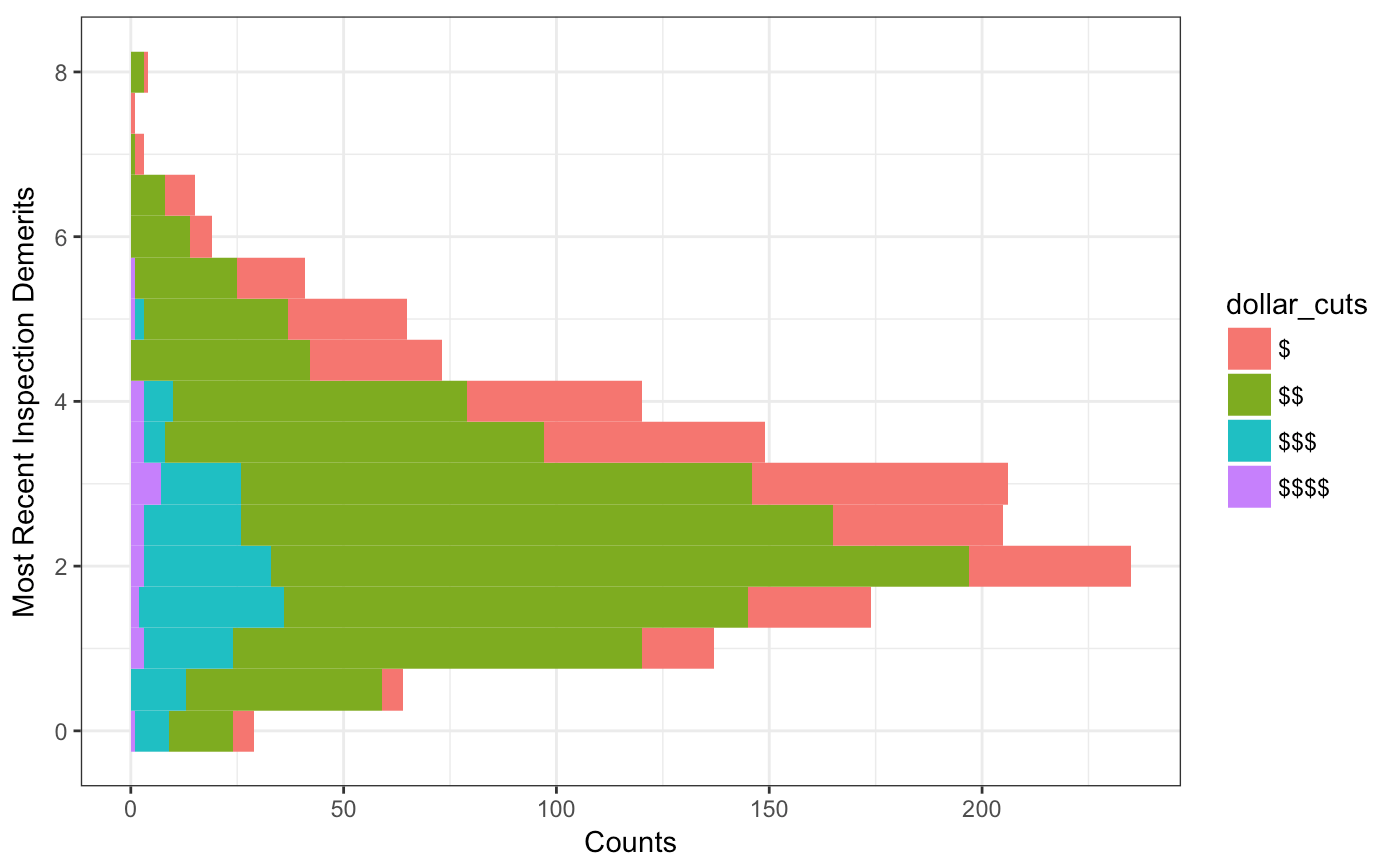
\includegraphics[scale = 0.3]{expensive}
    \caption{The relationship between expensiveness and averaged violation counts. }
\end{figure}


%%%%%%%%%%%%%%%%%%%%%%%%%%%%%%%%%%%%%%%%%%%%%%%%%%%%%%%%%%%%%%%%%%%%%%%%%%%%%%%%

%%%%%%%%%%%%%%%%%%%%%%%%%%%%%%%%%%%%%%%%%%%%%%%%%%%%%%%%%%%%%%%%%%%%%%%%%%%%%%%%
\subsection*{2.3 Yelp Reveiws}

\subsection*{2.3.1 Sentiment Analysis}

The VADER (Valence Aware Dictionary and Sentiment Reasoner) model is a Python package developed mainly for sentiment analysis (Hutto \& Gilbert, 2014). VADER is based on lexicons of sentiment-related words and will produce four sentiment metrics: positive, negative, neutral and compound scores for the text message. The first three metrics each represent the proportion of the text that falls into those categories and the compound score is a summary score that ranges from -1 to +1 with negative score representing negative sentiment, vice versa.

In our analysis, we computed a sentiment matrix for every review and averaged the scores for each restaurant. As shown below in Figure 2, there is a trend that the compound score correlates negatively with the average number of past violations.

\begin{figure}[h]
	\centering
    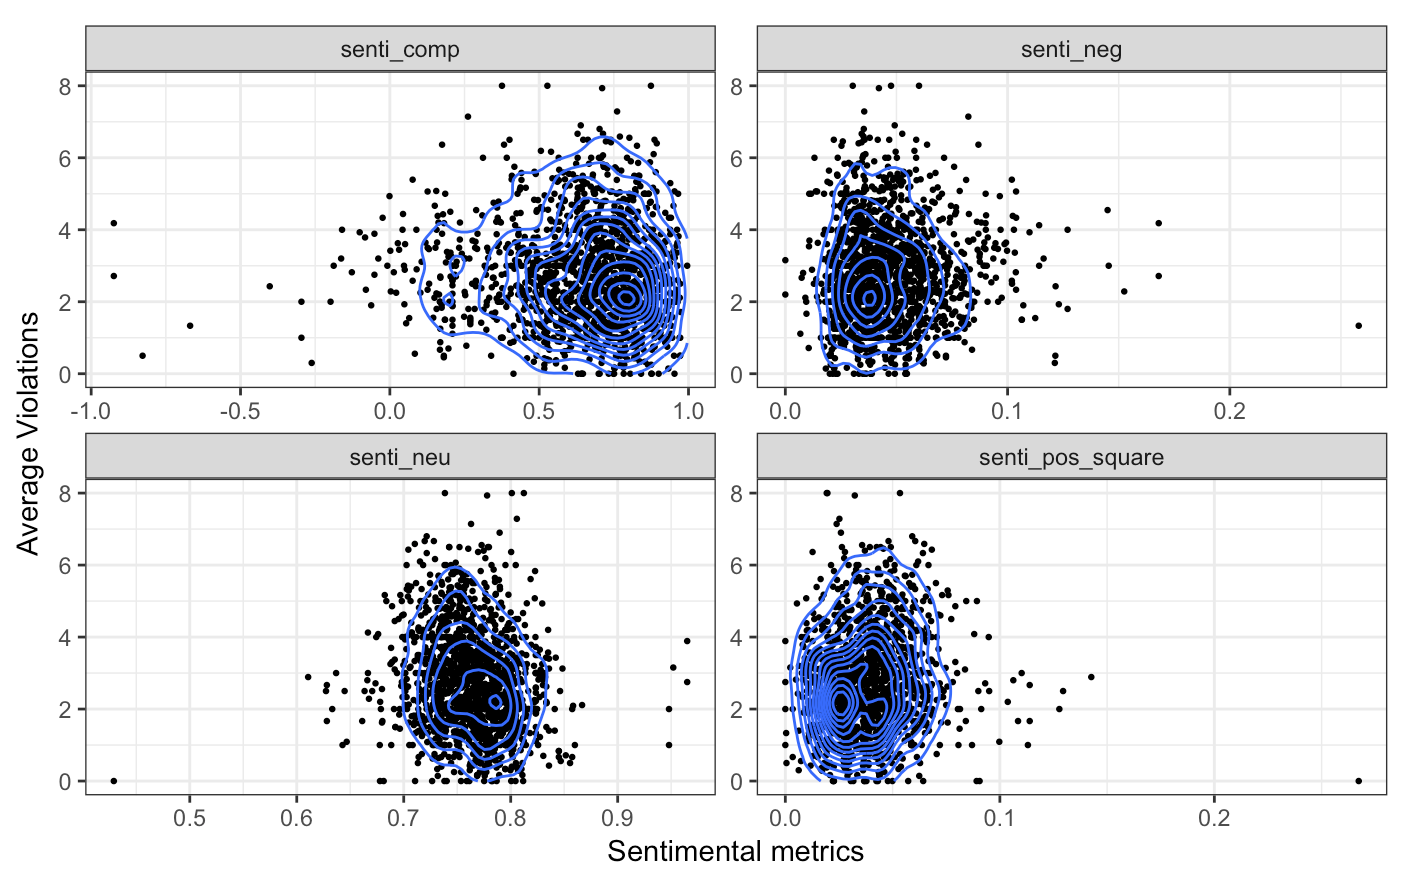
\includegraphics[scale = 0.3]{senti}
    \caption{The relationship between sentiment scores and number of violations}
\end{figure}

%%%%%%%%%%%%%%%%%%%%%%%%%%%%%%%%%%%%%%%%%%%%%%%%%%%%%%%%%%%%%%%%%%%%%%%%%%%%%%%%

\subsection*{2.3.2 Keyword Analysis}
In addition to the VADER model, we also defined a set of target keywords that is presumably related to health inspection. As can be seen in Figure 3 and 4, we have 15 subsets of keywords. All words within each subset have similar semantic meaning so that we can account for different users' wording habits. 

We also used useful counts and the length of the review as weights for the keywords. As one can imagine, not all Yelp users are very responsible when they leave a review. Therefore, the reviews that were agreed by others or are very long in the first place should be considered as more important. Because of the weights we used, the keywords counts are usually numerically very large. As a result, we used the log form of all the keyword counts while building models. 

\begin{figure}[h]
	\centering
    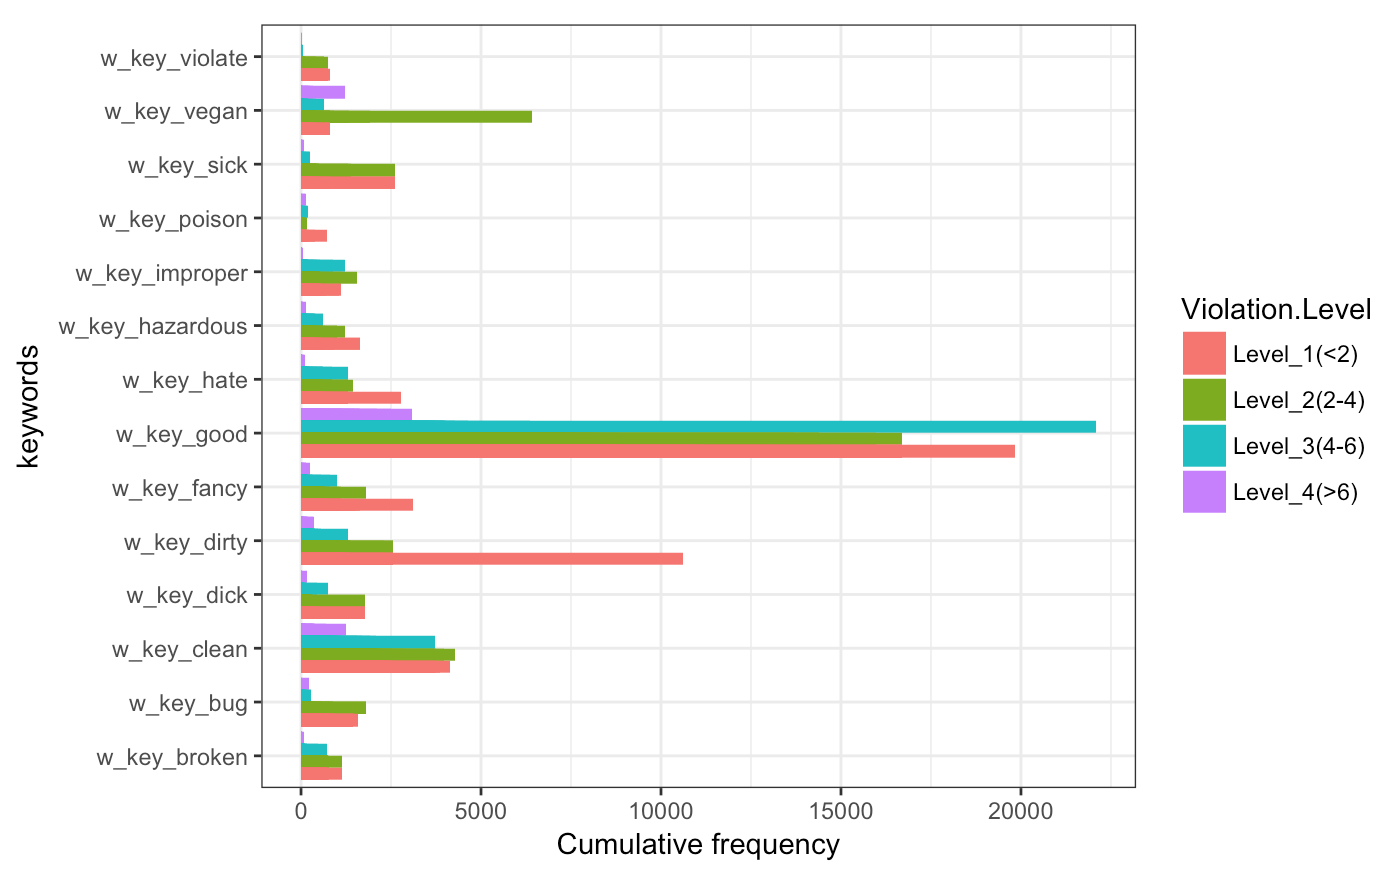
\includegraphics[scale = 0.3]{keyword}
    \caption{}
\end{figure}

Moreover, we also used the "$get\_word\_forms$" Python package to get possible verb or adjective forms of the keywords so that we could catch the keywords in different semantic settings. Similar to the VADER analysis, we first divided each review into individual words, then we check if that word is spelled correctly, if not, we found the first 5 most frequent guess of the correct form. Lastly, we checked if any of the words from the review are in the target set. We also multiplied the counts of each subset of the keywords by the number of hits on "usefulness" of the review so that popular reviews get a higher weight in the analysis. After we have the weighted counts for each subset of the keywords, we averaged those counts for each restaurant. 

\subsection*{2.4 Selected Features}
To sum up, Table 1 listed all the features we used in this project. 

\begin {table}
\caption {Feature Summary}
\begin{center}
	\tiny
	\begin{tabular}{l*{4}{c}r}
    \hline
	Source& Features\\
    \hline
    Inspection Dataset& $Grade A ratio,Latitude, Longitude$\\
    &$Latitude, Neighborhood, Reinspection Ratio$\\
    \hline
    & $Review Counts(log), Review Rating(log)$\\  &$Restaurant Category, senti\_comp, senti\_pos$\\ &$senti\_neu, , w\_key\_dirty$, senti\_neg \\
    Yelp.com&$w\_key\_good, w\_key\_clean, w\_key\_fancy$\\
    &$w\_key\_vegan, w\_key\_sick, w\_key\_hazardous$\\
    &$w\_key\_improper, w\_key\_hate$ \\
    &$w\_key\_dick, w\_key\_bug, w\_key\_broken, w\_key\_violate$ \\
    \hline
	\end{tabular}
\end{center}
\end{table}

Figure 8 presents a correlation matrix for most of the features involved (categorical features such as restaurant category and neighborhood are not included), along with the dependent variable. As we can see from the matrix, there are very few correlation between features so we didn't conduct any unsupervised learning to reduce the dimension of the feature space. 
Furthermore, we can also see that correlation coefficient between  Latitude/Longitude and the dependent variable is close to 0. Therefore, we remove these two features from the linear models. 
\begin{figure}[h]
	\centering
    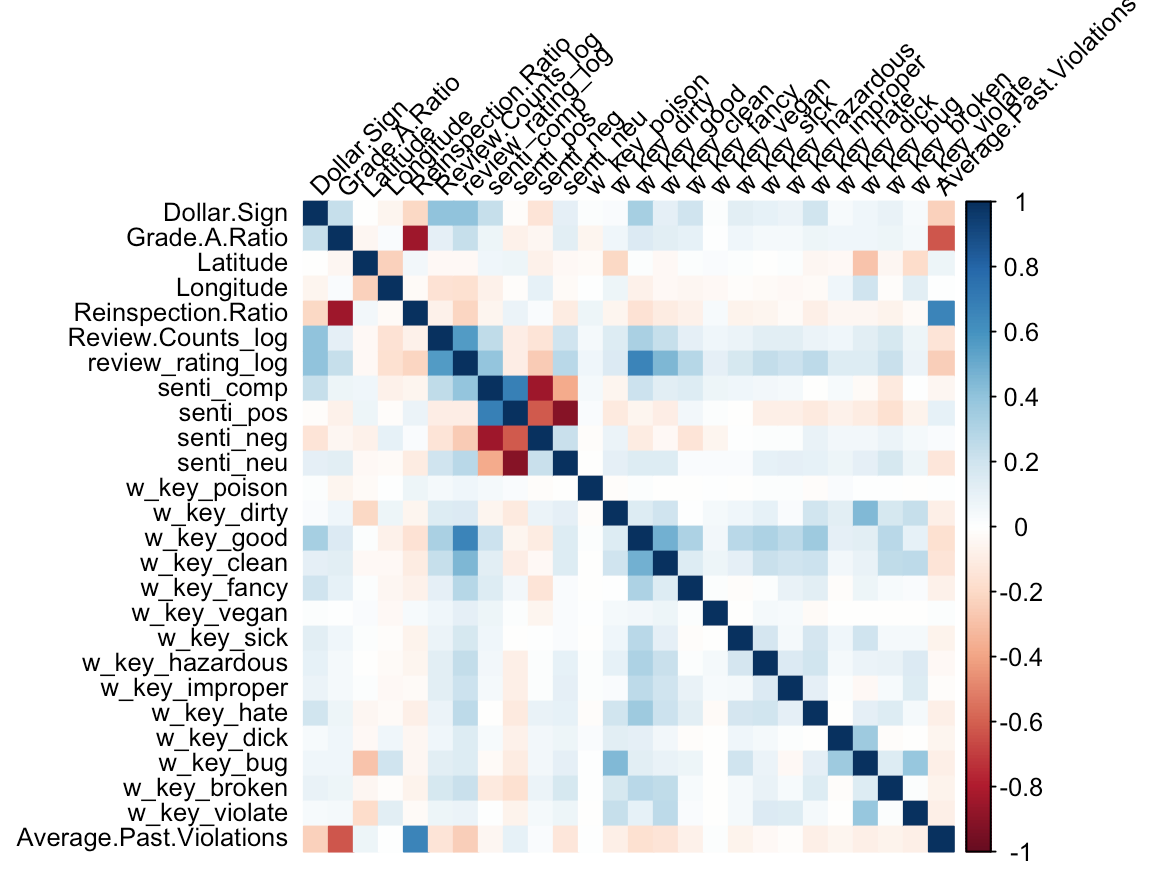
\includegraphics[scale = 0.4]{cor}
    \caption{Correlation between features and the number of violations}
\end{figure}

%%%%%%%%%%%%%%%%%%%%%%%%%%%%%%%%%%%%%%%%%%%%%%%%%%%%%%%%%%%%%%%%%%%%%%%%%%%%%%%%


\section*{3 Model Selection}

For the purpose of model selection, we randomly selected 20\% of the data to be the test set (384 data points in total) and the remaining 80\% (1540 data points) were used as training data. 

\subsection*{3.1 Linear Models}

We fitted linear regression models using different loss functions and regularizers, and get respective mean square errors on test dataset for comparison. Cross-validation method were used to decide the best parameter $\lambda$ on regularizers. 

According to the descriptive analysis, we don't have many outliers and the range of the dependent variable, averaged violation counts, is within the range 0-9. So we first consider Quadratic loss. For comparison, Huber loss is also used to check the robustness of the model. Quadratic regularizer was considered to lower the model variance. Having 49 features (including one-hot encoding category features) in total, we would like certain sparsity in the model. This implies the use of L1 regularizer. We first tried the quadratic loss without regularizer and then used the combination of Quadratic and Huber Loss and Quadratic and L1 regularizer were included in four models. 

To determine the parameter $\lambda$, we did the five-fold cross validation. Figure 9 displays the cross validation result for the model with Quadratic loss and L1 regularizer, which indicates $\lambda = 1$ can be used in this model.

The linear model with Quadratic loss and no regularizer has the least MSE. The scatter plot of true value and predicted values have similar shape to Figure 10, which indicates that linear model didn't well explained the variance of averaged violation counts. The result motivated us to explore more non-linear models next.

Quadratic Loss Function: \[ minimize\frac{1}{n}\sum_{i=1}^{n}  (y_i- w^T x_i)^2 +  r(w)\]

Quadratic Regularlizer: \[r(w) = ||W||^2 \]

Huber Loss Function: \[ minimize\frac{1}{n}\sum_{i=1}^{n} huber  (y_i- w^T x_i) +  r(w)\]

L1 Reaularlizer: \[  r(w) = \lambda \sum_{i=1}^{n}|w_i|\]
\begin{table} [h]
\caption {MSE for Linear Models}
\begin{center}[h]
	\tiny
	\begin{tabular}{l*{4}{c}r}
    \hline
	Loss Function & Regularlizer & Mean Square Error \\
    \hline
    Quadratic & No regularizer  & 2.15  \\ 
    Quadratic & L1  & 2.35  \\ 
 	Quadratic & Quadratic  & 2.46  \\  
 	Huber  & Quadratic  & 2.72  \\   
 	Huber  & L1  & 2.93  \\ 
    \hline
	\end{tabular}
\end{center}
\end{table}

\begin{figure}[h]
	\centering
    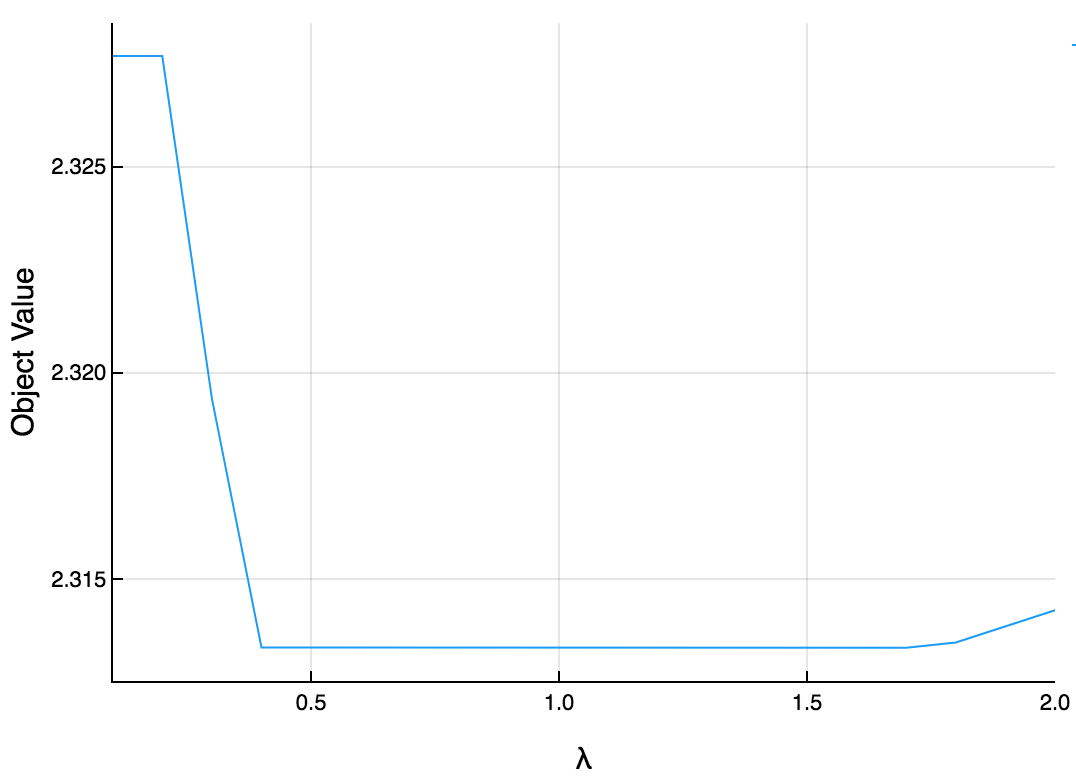
\includegraphics[scale = 0.35]{cv_l1}
    \caption{Cross validation of $\lambda$ in the model with Quadratic loss and L1 regularizer}
\end{figure}

\begin{figure}[h]
	\centering
    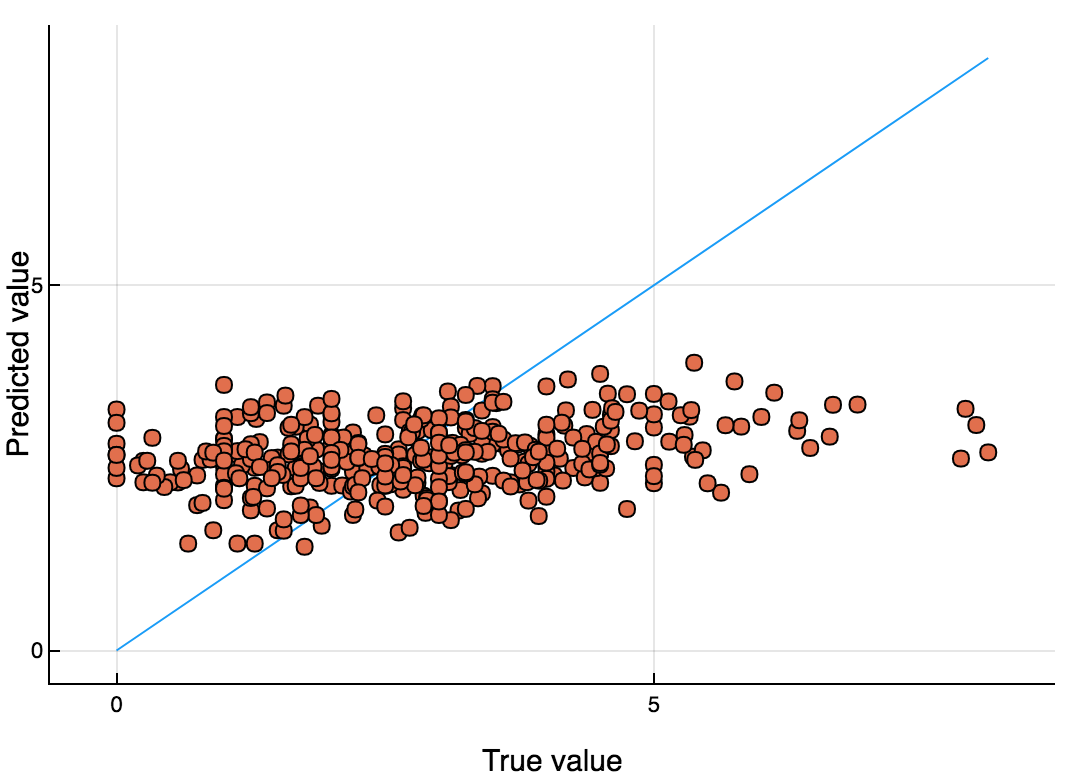
\includegraphics[scale = 0.35]{quad_noreg}
    \caption{The scatter plot of predicted violation counts and true violation counts with Quadratic loss and no regularizer}
\end{figure}


%%%%%%%%%%%%%%%%%%%%%%%%%%%%%%%%%%%%%%%%%%%%%%%%%%%%%%%%%%%%%%%%%%%%%%%%%%%%%%%%


\subsection*{3.2 Non-linear Models}

As we can see from the feature engineering section, some features don't necessarily have a linear relationship with the average number of violations. Thus, in addition to the linear models above, we also tried some nonlinear models. 
\subsection*{3.2.1 Random Forest}

The first non-linear model we trained is random forest. Random forest uses bootstrapping (AKA bagging) sampling method that constructs a multitude of decision trees during training time. This unique bagging sampling method produces many subsets of the original training data (but with possible repetitions of some single data points)and each of the decision trees involved works independently from each other. Just like any regular decision tree, the trees split on each feature aiming at maximizing the information we can gain from that split. When it comes to prediction, we take the mean prediction of all the trees and output one averaged decision tree. By doing so, we avoid the problem of over fitting. 

We used 10-fold cross validation to choose an optimal max depth of the tree for random forest model and compared averaged mean square error (MSE) for each max depth we tried (Figure 11). As you can see from the line chart, MSE reaches its minimum when the max depth is 6. Therefore, we build the model using a maximum depth of 6. 
\begin{figure}[h]
	\centering
    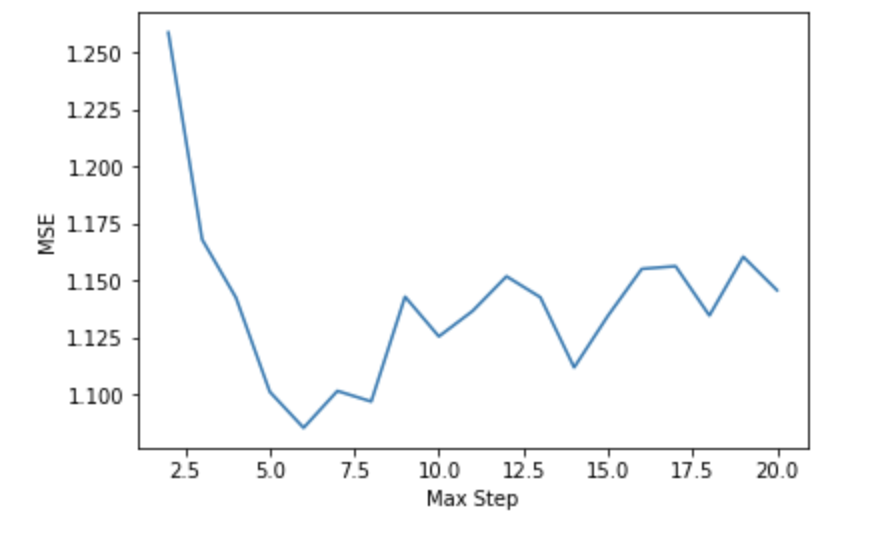
\includegraphics[scale = 0.55]{random_forest_cv_graph}
    \caption{Cross-Validation Result for Random Forest}
\end{figure}

The minimum MSE of random forest model is 1.08 and the relationship of observed value and predicted value is shown in Figure 12. 
\begin{figure}[h]
	\centering
    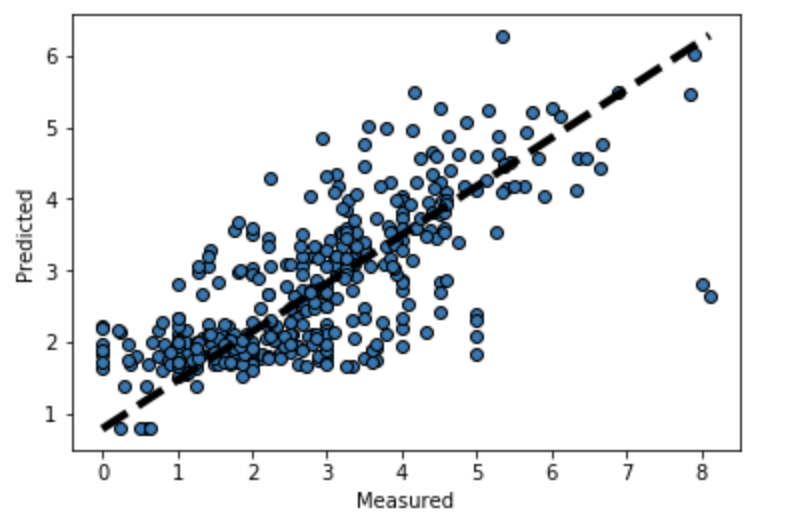
\includegraphics[scale = 0.6]{random_forest_result_updated}
    \caption{Random Forest's Predicted Value}
\end{figure}
We also compared the relative importance of the 10 most important features in the model we trained above. Shown in figure 13, we can see that the negative and composite sentiment score are the most important contributor to our model here, which means that Yelp reviews are very predictive of health inspection results. 
\begin{figure}[h]
	\centering
    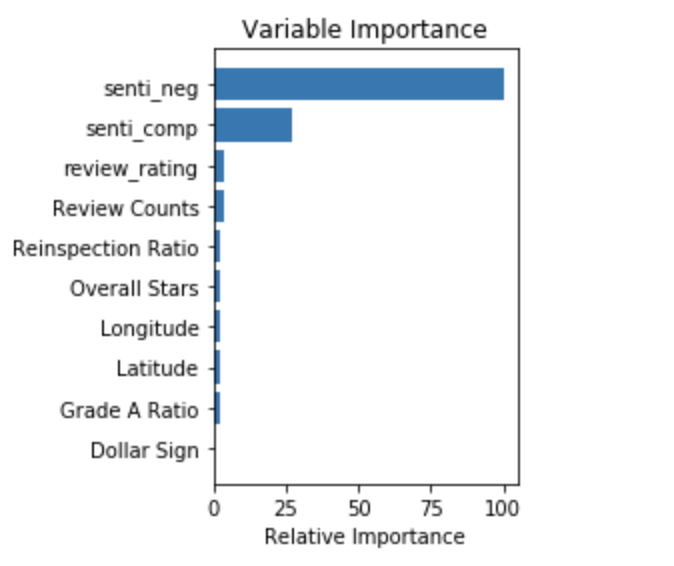
\includegraphics[scale = 0.7]{random_forest_features}
    \caption{Feature Importance for Random Forest}
\end{figure}

\subsection*{3.2.2 Gradient Boosting Regression}

In addition to random forest, we also trained a gradient boosting regression model with quantile loss function.

A gradient boosting regression model is typically used in decision trees and unlike random forest, which uses bagging sampling to reduce over fitting, the gradient boosting method builds model in a stage-wise fashion and it generalizes them by allowing optimization of an arbitrary differentiable loss function.

For the differentiable loss function, We specifically chose quantile regression here because in our case, a false positive result has a more severe consequences than a false negative (i.e. the model may predict a restaurant is good enough not to be inspected this year but it's actually not maintaining a healthy environment cause much more trouble for people than the model being too harsh and predict restaurants to be worse than they actually are). The quantile loss function calculates the loss as follows: 

Quantile Loss Function: \[ minimize\frac{1}{n}\sum_{i=1}^{n}  \alpha (y_i- w^T x_i)_+ + (1-\alpha) (y_i- w^T x_i)_- \]

Therefore, in order to penalize false positive more than false negative, we chose an $\alpha$ of 0.7, with 500 estimators and a max depth of 6 (same as the random forest model) to build a gradient boosted model. Furthermore, we used log(average number of past violations) before training the gradient boosted model because from the scatter plot, we can observe a exponential relationship between many of the features and the number of past violations. Therefore, we trained the model to fit the log transformation of the dependent variable and transformed it back before calculating MSE. 

After training the model, we tested it on the test data and  gives us a MSE of 1.25. As we can see in Figure 14, the deviance of training and testing error both decreased rapidly when the iteration first starts to increase and the deviations in both datasets began to stabilize. 
\begin{figure}[h]
	\centering
    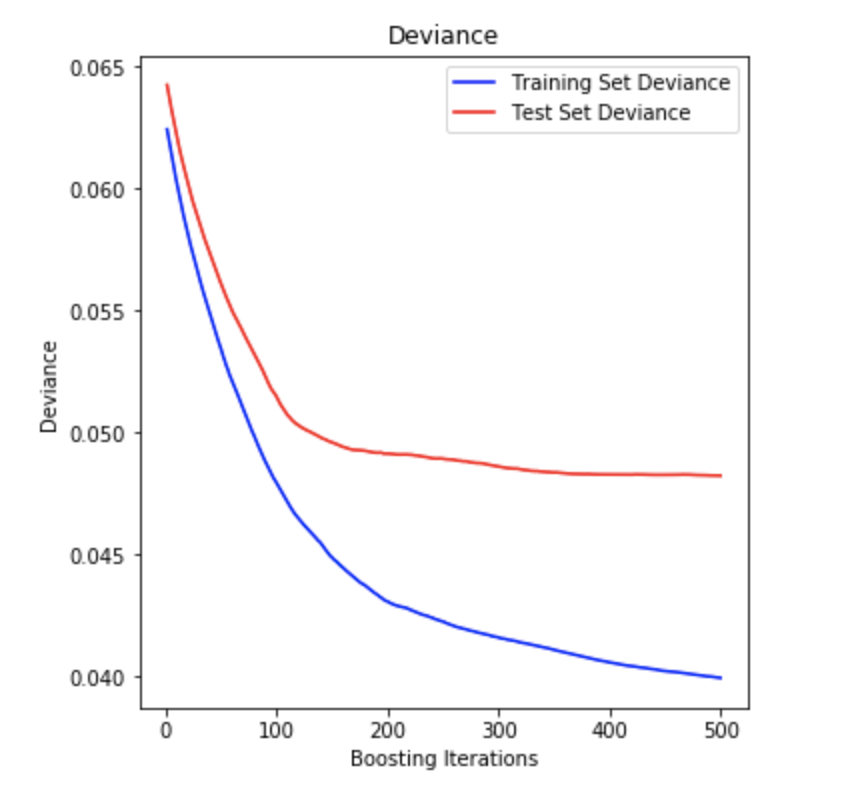
\includegraphics[scale = 0.6]{gradient_boosted_iterations}
    \caption{Deviation Trend for training and testing error}
\end{figure}
The predicted value of the gradient boosted model is shown in Figure 15 and the 10 most important features were shown in Figure 16. 
\begin{figure}[h]
	\centering
    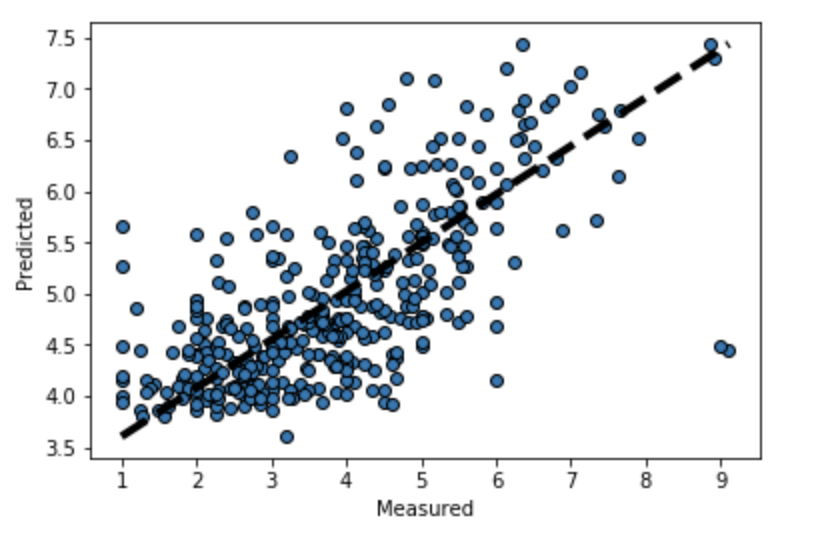
\includegraphics[scale = 0.6]{gradient_boosted_result}
    \caption{Gradient Boosted Model's Predicted Value}
\end{figure}

\begin{figure}[h]
	\centering
    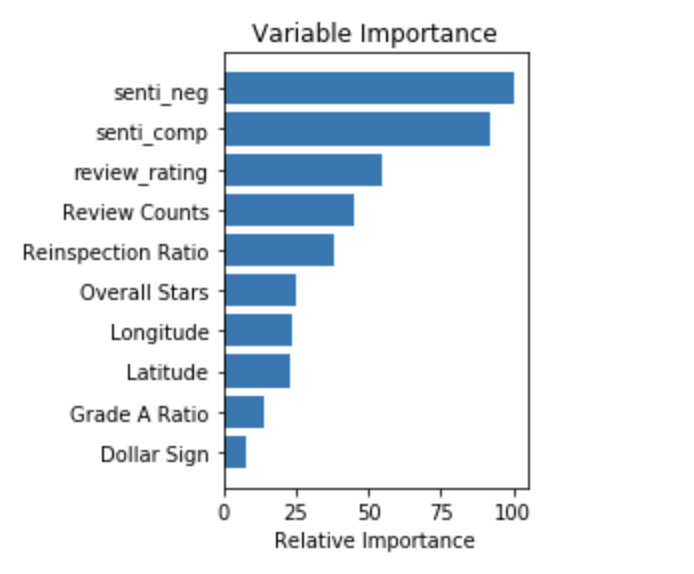
\includegraphics[scale = 0.6]{gradient_boosted_features}
    \caption{Feature Importance for Gradient Boosted Model}
\end{figure}

%%%%%%%%%%%%%%%%%%%%%%%%%%%%%%%%%%%%%%%%%%%%%%%%%%%%%%%%%%%%%%%%%%%%%%%%%%%%%%%%
\newpage
\section*{4 Results}
To sum it up, the MSE of all the models we trained are shown in Table 2. As can be seen from the table, if we want to pick a model with the smallest test error, we should pick random forest. However, as we mentioned before, the problem of interest here is to use Yelp data to provide general public and the health department with some insights in terms of whether a restaurant is healthy enough. Therefore, we would want to avoid false positive. While the gradient boosted model with quantile regression's MSE (1.25) is reasonably small as well. Thus, in consideration of practical implications, we recommend using the gradient boosted model with quantile regression. 

\begin {table}[h]
\caption {MSE for Models}
\begin{center}
	\tiny
	\begin{tabular}{l*{4}{c}r}
    \hline
	Model Type& Model Name & MSE\\
    \hline
    Linear& Quadratic Loss function with Quadratic regularizer& 2.46\\
    Linear& Quadratic Loss function with l1 regularizer& 2.35\\
    Linear& Huber Loss function with Quadratic regularizer& 2.72\\
    Linear& Huber Loss function with l1 regularizer& 2.93\\
    Non-linear & Random forest & 1.08 \\
    Non-linear & Gradient Boosted Model with Quantile Loss function & 1.25 \\
    \hline
	\end{tabular}
\end{center}
\end{table}


%%%%%%%%%%%%%%%%%%%%%%%%%%%%%%%%%%%%%%%%%%%%%%%%%%%%%%%%%%%%%%%%%%%%%%%%%%%%%%%%

\section*{5 Discussion}
We aimed to use features from Yelp.com to predict restaurants' health inspection result. By using feature engineering techniques such as one-hot-encoding, log transformation and natural language processing, we compared regression results from four linear models and 2 non-linear models. In the end, we were able to minimize the test error (i.e. MSE) to be less than 1.5.

For the purpose of practical implications, we believe gradient boosted regression with quantile loss function is the most suitable one for predicting how many violations a restaurant has in the past few years. As you can see from the results of gradient boosted model, the most important four features all came from Yelp reviews, which indicates that Yelp reviews can provide useful insights for the restaurant's healthy level. Another interesting result of the model is that the overall star from Yelp is useless when compared to the weighted rating we computed from the reviews, which means that the overall star is not informative and may contain a lot of Spam since it's cumulative and can be biased.  

Though our model did reasonably well in terms of predicting the health inspection results, one should be careful when they apply the model in other settings. First of all, all the datasets we used here were from Las Vegas and different states in the US can have various standards about health inspection. Secondly, as we said before, healthy eating is a very serious issue and false positives can cause serious consequences. Therefore, people should be critical when they use any kind of healthy measure when choosing different restaurants. 

%%%%%%%%%%%%%%%%%%%%%%%%%%%%%%%%%%%%%%%%%%%%%%%%%%%%%%%%%%%%%%%%%%%%%%%%%%%%%%%%

\section*{Reference}
Gilbert, C. H. E. (2014). Vader: A parsimonious rule-based model for sentiment analysis of social media text. In Eighth International AAAI Conference on Weblogs and Social Media.

\end{document}